\chapter{Fundamentals}
\section{Go}
Go (also known as Golang) is an open source programming language that was started at Google in 2007 and initially launched in 2009.
The language was designed to face engineering challenges at Google with the goal to make it \enquote{easy to build simple, reliable and efficient software}. \cite{pike.2020, golang.github}
By now, the compiled and statically typed language \cite{chris.2021} is widely used and the way it approaches network concurrency and software engineering has influenced other languages to a noticeable extent. \cite{pike.2020}
Through its structure go supports programming on various levels of abstraction.
For instance, one can embed Assembler or C code into a Go program or on the other hand combine groups of components into bigger, more complex components to realize abstract design patterns. \cite{Maurer2021}
Nowadays, Go is a popular choice for everything related to DevOps and therefor also for the development of command line tools. \cite{mike.2020}

Go also tries to provide its own, official solutions for common tasks in software development.
When installing Go, it comes packed alongside with a formatter (which shall ensure uniform styling across all programs written in Go) and an included suite for unit testing, just to name a few examples.
Furthermore, Go supports generating documentation based on comments in the source code; much alike JavaDoc.
Go features an extensive standard library which depicts a good starting point for developing your own applications.
In case one wants to include a third party library, this can be done via the \emph{go get} command.
It fetches the necessary resources (usually directly from a \ac{vcs}) and saves the modules as a dependency in the \emph{go.mod} file. \cite{go.tour, go.docs}

% \begin{itemize}
%     \item toolchain (uniform formatter, included test suite, source code based generation of documentation)
%     \item third party modules repo / go get
%     \item extensive standard library
%     \item (cite from golang.org tutorial)
% \end{itemize}

% started in 2007 released in 2009
% open source, compiled, and statically typed programming language (https://www.freecodecamp.org/news/what-is-go-programming-language/)
% face engineering challenges at Google (https://go.dev/solutions/google/)
% goals: make it "easy to build simple, reliable and efficient software" (https://github.com/golang/go)
% by now widely used
% network concurrency and software engineering are influencing other languages (https://go.dev/solutions/google/)
% through its structure go supports programming on various layers of abstraction (cite from book here)
%     supports embedded assembler and c
%     suitable for realizing abstract design patterns

\subsection{Cobra}
Cobra is an open source library for Go.
Its aim is to provide developers with an easy way to create modern \ac{cli} applications.
The cobra library is being used by noticeable projects like the \ac{cli}s for Kubernetes or for GitHub.
The idea behind Cobra's intended command schema is that commands of a well constructed \ac{cli} should read like sentences.
This way, new users that are familiar with \acp{cli} in general quickly feel native because interacting with the \ac{cli} feels more natural.
In this approach, a command represents a certain action that the \ac{cli} can perform.
This action than take arguments and flags to further specify on which objects and in which way the command should take action.
With Cobra, one can also easily create nested subcommands.
This means that a before mentioned command can also be divided into multiple sub-actions to enable detailed handling of complex actions.
Further, benefits of Cobra are, among others, the automated generation of autocompletion for the most common shells as well as the ability to automatically create man pages. \cite{cobra.github, cobra.dev}


% \begin{itemize}
% 	\item open source library
%     \item modern cli applications
%     \item "namenhafte" projects like Kubernetes, GitHub CLI
%     \item subcommand-based -> explain
%     \item nested subcommands
%     \item can automatically generate autocomplete
%     \item helps in generating man pages \cite{cobra.github}
% \end{itemize}

\section{Kubernetes}
\label{sec:kubernetes}
Kubernetes (often short: k8s) is an open source solution to ease up and automate management of container based services.
It follows a declarative paradigm.
This means that the user just needs to describe the desired state -- for example through the use of configuration files or via the Kubernetes \ac{cli} -- and Kubernetes determines the steps by itself which are necessary to reach and maintain this state.
Kubernetes also enables users to dynamically scale their applications and services.
This means that the amount of resources, that are dedicated to an application, is adapted during runtime dependent, for example, on the current number of users.
Furthermore, Kubernetes can perform load balancing and redundancy between different instances of the same service.
\cite{Bloß2019, wasistk8s}

One instance of a Kubernetes system is called a cluster.
A Cluster is composed of multiple nodes (which usually are virtual machines or physical servers) which run the actual applications.
An Application runs inside some kind of container, internally called Pod.
The interaction with a cluster is managed by the so-called \emph{Kubernetes Master}.
It is a central controlling unit.
The user actually never interacts with the nodes themselves directly.
\cite{k8skonzepte}

\section{Gardener}
Even though there are tools that help with creating and updating single Kubernetes clusters, it is rather hard to manage many clusters.
This is where Gardener comes into play.
It is a Kubernetes native extension that manages Kubernetes clusters as a service, packing the performance to manage up to thousands of clusters.
One key concept that is applied is so-called self-hosting.
This means that Kubernetes components are run inside of Kubernetes clusters and is done, because Kubernetes is the go-to way to easily manage software in the cloud. \cite{gardener.architecture, gardener.blog1, gardener.blog2, gardener.cloud}

Gardener's architecture is constructed much like Kubernetes itself although not individual Pods are managed but entire clusters.
The root of all is the so-called \emph{Garden Cluster}.
It is the main interface for the Gardener administrator and hosts, among others, the Garden Cluster control plane, the Gardener dashboard, the Gardener \ac{api} server, the Gardener controller manager and the Gardener scheduler.
Then there are two other types of clusters, \emph{Seed Clusters} and \emph{Shoot Clusters}.
One Seed Clusters manages the control planes (thus \ac{api} server, scheduler, controller manager, machine controller etc.) of its Shoot Clusters.
There is at least one Seed Cluster per \ac{iaas} provider and region.
The Shoot Clusters control planes are deployed as Pods inside the Seed Cluster and can therefore be created with standard Kubernetes deployment and support rolling updates.
Shoot Clusters only contain worker nodes and are the Kubernetes Clusters that actually become available to the end-user and can be ordered in a declarative way.
The clusters created by Gardener are vanilla Kubernetes clusters independent of the underlying cloud provider. \cite{gardener.blog2, wasistgardener}
(More details of the described architecture can be seen in \autoref{fig:gardener-architecture}.)

\begin{figure}[H]
    \centering
    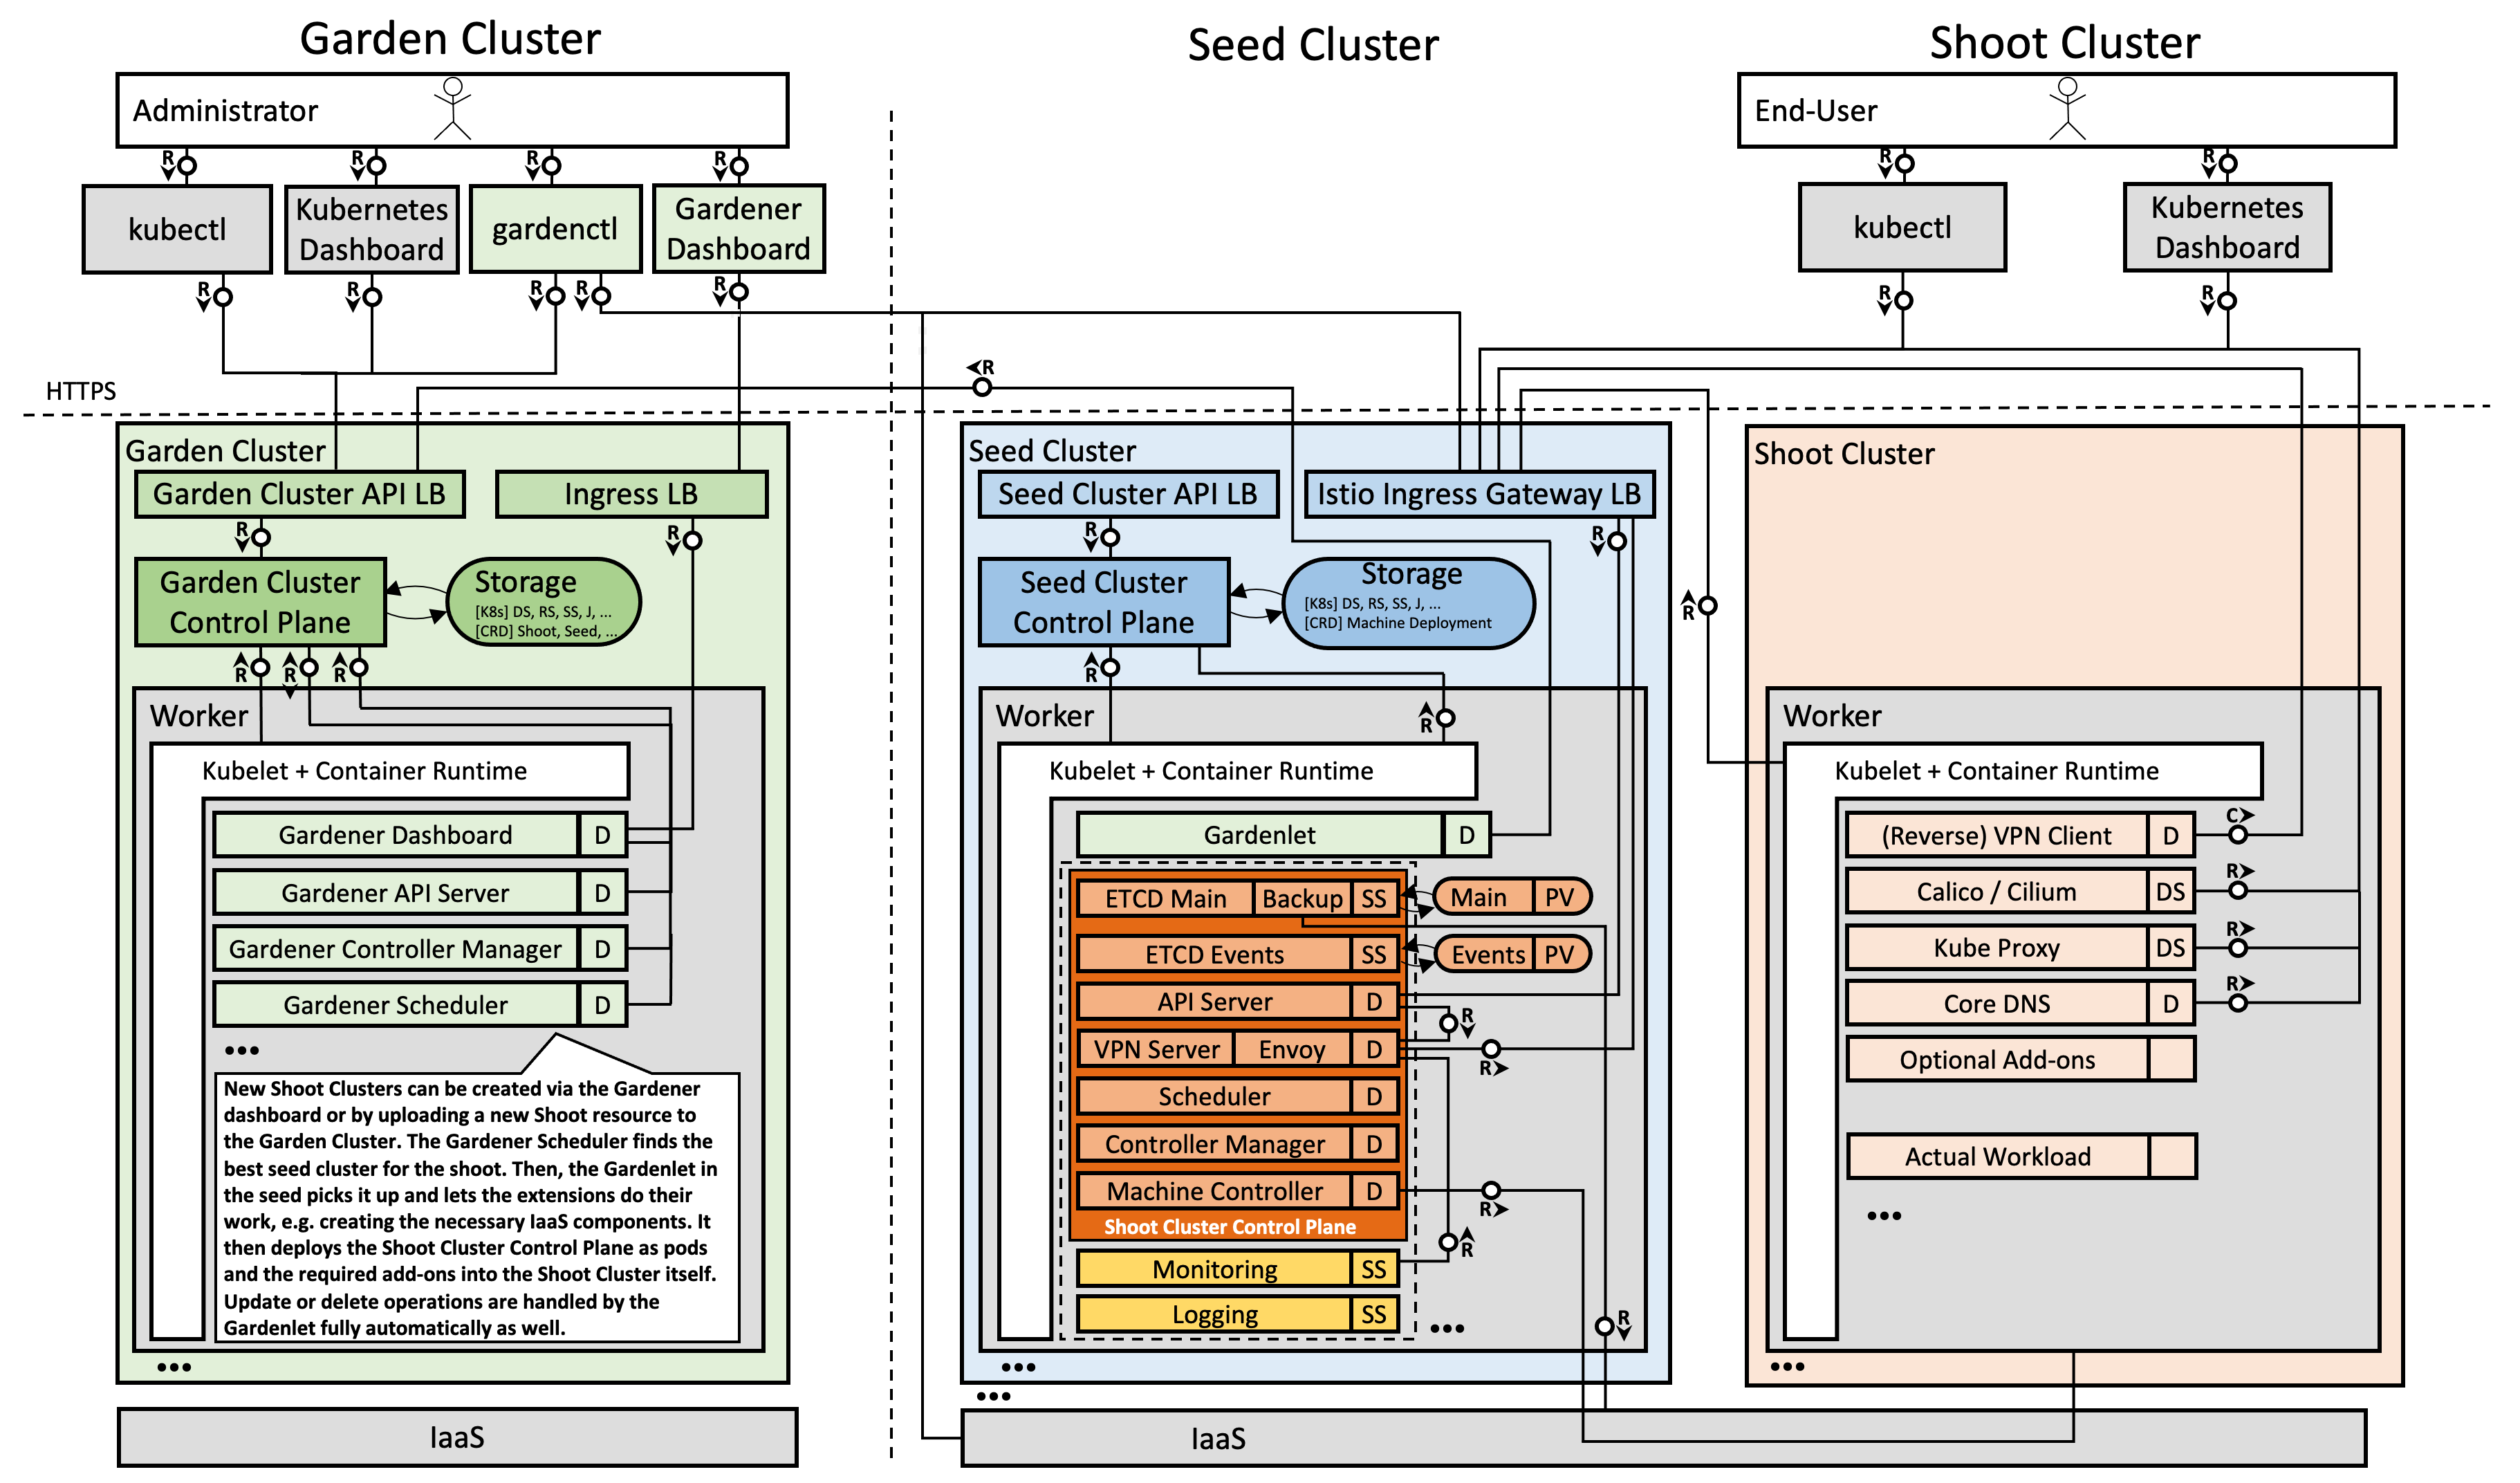
\includegraphics[width=\textwidth]{Bilder/gardener-architecture-detailed.png}
    \caption{Gardener architecture \cite{gardener.architecture}}
    \label{fig:gardener-architecture}
\end{figure}

% \begin{itemize}
%     \item open source software by SAP
%     \item for managing Kubernetes cluster (Kubernetes as a service)
%     \item Kubernetes native extension
    
%     \item cite https://kubernetes.io/blog/2018/05/17/gardener/
%     \item Even though there are tools that help with creating and updating single Kubernetes clusters, it is rather hard to manage many clusters.
%     \item there are tools to help in creating and updating single Kubernetes clusters
%     \item but very hard to manage many clusters
%     \item this is the focus of Gardener
%     \item manages Kubernetes clusters as a service
%     \item Gardener creates Kubernetes-conformant clusters
%     \item supports deployment to multiple cloud providers
%     \item brings the ability to manage thousands of clusters
%     \item 
% \end{itemize}

\section{\ac{aws}}
\acf{aws} is a subsidiary company of Amazon that offers a cloud computing platform with various services, such as \ac{s3} \cite{aws.s3} or \ac{eks} \cite{aws.eks}.
Started in 2006, \ac{aws} nowadays runs data centers all over the world to provide scalable, reliable, and high performing services. \cite{aws.linkedin, whatisaws}

At the time of writing, \ac{aws} is the cloud provider with the biggest market share. \cite{aws.marketshare}
Also, most of the supervising department's clusters are currently being deployed on \ac{aws}.
Because of these reasons and also due to constraints in time and complexity, the bootstrapping process worked out in this report is going to be narrowed down to deployment in an \ac{aws} environment.

\section{Terraform}
Modern enterprise infrastructure for software development usually makes use of cloud computing to dynamically adapt infrastructure to the fast-paced world of agile development.
These clusters are usually distributed between multiple cloud services, each of which uses their own individual \acp{api} to configure their platform.
Terraform is a tool that tries to minimize the effort needed to deploy these infrastructures in the long run by automating resource management as far as possible.
It allows to uniformly describe the target infrastructure in an easy to learn, machine-readable definition language and automatically takes care of deploying this infrastructure at the individual \ac{iaas} providers.
This approach is also known as \ac{iac}.
With Terraform, it is also possible to save provisioned infrastructure setups as a Terraform configuration to reuse them at a later point in time or to arbitrarily extend and adapt the configuration.
For configuration, either \ac{json} or \ac{hcl} can be used, with \ac{hcl} being the preferred way by the developing company HashiCorp because of its advanced features compared to \ac{json}.
Terraform can only unleash its full potential because of cooperations with all major software and hardware vendors and providers.
HashiCorp partners with over 160 companies and services the most noticeable ones being:
\begin{itemize}
    \item \ac{aws},
    \item Atlassian,
    \item Cloudflare,
    \item Google,
    \item Microsoft, and
    \item Oracle.
\end{itemize}

The most common use cases for Terraform include general \ac{iac}, managing Kubernetes (\autoref{sec:kubernetes}), multi-cloud deployment, management of network infrastructures, and management of virtual machine images.
Terraform additionally integrates tightly with other HashiCorp services like Vault (\autoref{sec:vault}).

% \begin{itemize}
%     \item codifies cloud apis into declarative configuration files
    
%     \item minimiert langfristig den für das Deploment benötigten Aufwand
%     \item um den modernen Ansprüchen der Schnelllebigkeit gerecht werden zu können, müssen IT-Administratoren Ressourcenmanagement weitmöglichst automatisieren
%     \item Kluster mit maschienenlesbaren Konfigurationscode beschreiben -> Infrastructure as Code
%     \item Terraform ermöglicht einheitliche Beschreibung von Zielinfrastruktur und sorgt für Umsetzung bei IaaS-Providern
%     \item erlaubt es, provisionierte Infrastruktur-Setups zu speichern, um diese zu einem späteren Zeitpunkt erneut nutzen oder beliebig erweitern/anpassen zu können
%     \item 160 Partner, sind unter anderem AWS, Atlassian, Cloudflare, Google, Microsoft und Oracle
    
%     \item üblicherweise wird auf verschiedene Cloud-Services zurückgegriffen um Infrastruktur für die Software-Entwicklung zu realisieren
%     \item daher menge verscheidedner Schnittstellen
%     \item mit Terraform aber nicht
%     \item statt individueller schnittstellensprache konfiguration über json oder HashiCorp Configurration Language (HCL)
%     \item hcl erlaubt kommentare und weitere features gegenüber json
    
%     \item Zusammenarbeit mit allen wichtigen Software und Hardware-Providern
    
%     \item häufige Anwendungsfälle für Terraform:
%     \item Infrastructure as Code
%     \item Multi-cloud deployment
%     \item Manage Kubernetes
%     \item Netzwerkinfrastruktur verwalten
%     \item Images von virtuellen Maschinen verwalten
%     \item Integration mit anderen HashiCorp Plattformen wie Vault
    
%     \item cite https://www.ionos.de/digitalguide/server/tools/was-ist-terraform/
%     \item cite https://www.terraform.io/
% \end{itemize}

\section{Jenkins}
Jenkins is a widely used open source automation server build with Java.
It is a \ac{cicd} tool aiming to save time by automating repetitive tasks like building projects, running test sets and deployment.
Jenkins supports many plugins (over 1800) via its update center which give you the ability to integrate with most of the common tools in development and automate practicably any project.
Jenkins can also be deployed on multiple machines to spread load and ensure quick and efficient operation.
\cite{jenkins.io, jenkins.github, gitlab.cicd}

In context of this project, Jenkins will be used after the successful bootstrap to take care of running Terraform and performing the actual deployment.

% \begin{itemize}
%     \item widely used open source automation server
%     \item built with Java
%     \item CICD tool (Continuous Integration and Continuous Delivery)
%     \item save time by automating repetitive tasks
%     \item like building projects, running tests and deployment
%     \item support for many plugins (over 1800) with its update center
%     \item give you the ability to deploy and automate any project
%     \item can be deployed on and spread load across multiple machines
%     \item cite https://www.jenkins.io/
%     \item cite https://github.com/jenkinsci/jenkins
    
%     \item 
% \end{itemize}

\section{Vault}
\label{sec:vault}
Vault is an open source service with the primary task to provide a central control unit to manage and organize enterprise secrets.
It encrypts secrets both at rest and in transit.
Access to the secrets can be granted granular per user through the use of \acp{acl}.
Furthermore, Vault audits access to the secrets.
That means that it keeps a detailed log on whom accessed what secret at which point in time.
If there was a security breach, where an unauthorized person got access to Vault, this protocol can be used to tell, if a specific secret has been read by the attacker or if it is still safe to use.

Vault is designed to be highly pluggable.
An instance is composed of \emph{storage backends}, \emph{audit log instances}, \emph{authentication providers} as well as \emph{secret backends}.
Each of these can be impersonated by a variety of different components.
This makes it possible to use different trusted authorities for attestation of identity.
For example, among others LDAP, JWT, GitHub, and Radius can be used.
An automated build service could very well use a different service to authenticate to Vault than a human user.

Secrets and encryption are often the weak spot in applications.
If a secret gets leaked and the leak stays unnoticed, attackers could gain long term access to a system.
As a solution, Vault offers \emph{dynamic secrets}.
When a client requests the access credentials for a supported system, Vault creates a short-lived secret just for that specific client.
Because the client is only accessing Vault, it does not have to bother with key creation nor rotation and an increased layer of security is added by not using secrets for an extended period of time.
Also, if a dynamic secret gets leaked, this single secret can be revoked individually.
If all clients accessing the resource used the same credentials, changing or blocking those could potentially cause an outage of the whole system.

When it comes to encryption, it can happen rather quickly that a single mistake compromises the security of the whole application.
Because of this, Vault offers encryption as a service.
The idea is, that Vault concentrates on the single task to handle credentials and encryption safely.
The broad variety of applications have a different focus and are not developed with the necessary expertise to guarantee safe implementation of security measures.
Vault, on the other hand, uses implementations that are audited by the open source community as well as independent experts.
Those are then provided as a high level \ac{api} to application developers.
That way, the encryption process of data gets very easy while, at the same time, Vault can handle the used encryption keys directly, and they are never actually sent to the application itself. \cite{vaultproject.io}

During the bootstrap, this project is about, a technical user is created for Terraform operations.
An access key is created for this user and then saved to Vault.
This way Jenkins then can obtain this access key and use it to run the actual cluster deployment with Terraform.

% \begin{itemize}
%     \item manage and organize secrets
%     \item provide a central secret storage
%     \item encrypt secrets at rest and in transit
%     \item ACL
%     \item Audit; log who has access what and when
%     \item a secret is a set of different credentials
%     \item protect sensitive data
%     \item various authentication methods; like LDAP, JWT, GitHub, Radius
%     \item authenticate against trusted sources of identity
%     \item trusted authority for attestation of identity
%     \item automate key issuance and rotation
    
%     \item dynamic secrets
%     \item create secrets for each specific client with limited lifetime
%     \item revoke a specific secret targeted
    
%     \item encrypt as a service
%     \item named key
%     \item high level API to do cryptography (encrypt, sign, verify, ...)
%     \item key and encryption logic never actually gets to the developer
%     \item control key lifecycle safely
%     \item protect application data at rest
    
%     \item highly pluggable
%     \item storage backends
%     \item Audit log instances
%     \item auth
%     \item secret backends (key/value, DB plugins, AWS, ...)
%     \item all of these are modular and can use solutions of various providers
    
%     \item cite https://www.vaultproject.io/
% \end{itemize}
